\documentclass{article}

% content/resources/templates/preamble.tex
\usepackage[margin=0.6in]{geometry}
\author{Milav Dabgar}
\usepackage{amsmath,amssymb,amsthm}
\usepackage{booktabs}
\usepackage{multirow}
\usepackage{xcolor}
\usepackage{tcolorbox}
\tcbuselibrary{breakable,skins}
\usepackage[colorlinks=true,linkcolor=blue]{hyperref}
\usepackage{titlesec}
\usepackage{enumitem}
\usepackage{tikz}
\usepackage{pgfplots}
\usepackage{circuitikz}
\usepackage[version=4]{mhchem}
\usepackage{longtable}
\usepackage{array}
\usepackage{float}
\usepackage{caption}
\usepackage{listings}

\lstset{
  basicstyle=\small\ttfamily,
  breaklines=true,
  breakatwhitespace=false,
  postbreak=\mbox{\textcolor{red}{$\hookrightarrow$}\space},
  float=false,
  numbers=left,
  numberstyle=\tiny\color{gray},
  numbersep=10pt,
  xleftmargin=2em,
  keywordstyle=\color{blue},
  commentstyle=\color{green!60!black},
  stringstyle=\color{purple},
  backgroundcolor=\color{gray!5},
  showstringspaces=false,
  tabsize=2,
  captionpos=b,
  keepspaces=true,
  columns=flexible
}

\pgfplotsset{compat=1.18}
\usetikzlibrary{shapes,arrows,positioning,calc,patterns,decorations.pathmorphing,decorations.markings,arrows.meta}

% Color scheme
\definecolor{headcolor}{RGB}{0,102,204}
\definecolor{keycolor}{RGB}{220,20,60}
\definecolor{solutioncolor}{RGB}{34,139,34}
\definecolor{mnemoniccolor}{RGB}{148,0,211}
\definecolor{codecolor}{RGB}{0,0,100}

% Spacing
\setlength{\parskip}{3pt}
\setlist[itemize]{nosep}
\setlist[enumerate]{nosep}

% Title formatting
\titleformat{\section}{\Large\bfseries\color{headcolor}}{\thesection}{1em}{}
\titleformat{\subsection}{\large\bfseries\color{headcolor}}{\thesubsection}{1em}{}

% Pandoc tightlist compatibility
\providecommand{\tightlist}{%
  \setlength{\itemsep}{0pt}\setlength{\parskip}{0pt}}

% Pandoc longtable compatibility
\newcounter{none}
\def\thenone{}


% content/resources/templates/english-boxes.tex

% Custom environments
\newtcolorbox{solutionbox}{
 breakable,
 enhanced,
 colback=solutioncolor!5!white,
 colframe=solutioncolor!75!black,
 fonttitle=\bfseries,
 title=Solution
}

\newtcolorbox{solutionboxnobreak}{
 colback=solutioncolor!5!white,
 colframe=solutioncolor!75!black,
 fonttitle=\bfseries,
 title=Solution
}

\newtcolorbox{keyformula}{
 breakable,
 enhanced,
 colback=keycolor!5!white,
 colframe=keycolor!75!black,
 fonttitle=\bfseries,
 title=Key Formula
}

\newtcolorbox{mnemonicboxenv}{
 breakable,
 enhanced,
 colback=mnemoniccolor!5!white,
 colframe=mnemoniccolor!75!black,
 fonttitle=\bfseries,
 title=Mnemonic
}

\newcommand{\mnemonicbox}[1]{%
  \begin{mnemonicboxenv}
    #1
  \end{mnemonicboxenv}
}


% Custom commands for GTU solutions
% This file defines semantic commands for consistent formatting

% Question command with automatic formatting
\newcommand{\question}[2]{%
  \section*{Question #1}%
  \textbf{#2}%
}

% OR question variant
\newcommand{\questionor}[2]{%
  \section*{Question #1 OR}%
  \textbf{#2}%
}

% Proper table environment with caption
\newenvironment{answertable}[1]{%
  \begin{table}[htbp]
  \centering
  \caption{#1}
}{%
  \end{table}
}

% Proper figure environment for diagrams
\newenvironment{answerdiagram}[1]{%
  \begin{figure}[htbp]
  \centering
  \caption{#1}
}{%
  \end{figure}
}

% Semantic markup for key terms
\newcommand{\keyword}[1]{\textbf{#1}}
\newcommand{\code}[1]{\texttt{#1}}
\newcommand{\classname}[1]{\texttt{#1}}
\newcommand{\methodname}[1]{\texttt{#1}}

% Proper quotation marks
\newcommand{\mnemonic}[1]{``#1''}


\title{Fundamentals of Electrical Engineering (4311101) - Winter 2023 Solution}
\date{January 19, 2023}

\begin{document}
\maketitle

\questionmarks{1(a)}{3}{Define Power \& Energy.}

\begin{solutionbox}
\textbf{Answer}:

\begin{itemize}
    \item \keyword{Power}: Rate of doing work or energy consumption per unit time. Measured in Watts (W).
    \item \keyword{Energy}: Ability to do work or the work done. Measured in Joules (J) or Watt-hours (Wh).
\end{itemize}

\begin{center}
\captionof{table}{Power vs Energy}
\begin{tabulary}{\linewidth}{|L|L|L|L|}
\hline
\textbf{Parameter} & \textbf{Definition} & \textbf{Formula} & \textbf{Unit} \\ \hline
\textbf{Power} & Rate of energy transfer & $P = W/t$ & Watt (W) \\ \hline
\textbf{Energy} & Capacity to do work & $E = P \times t$ & Joule (J) or Watt-hour (Wh) \\ \hline
\end{tabulary}
\end{center}
\end{solutionbox}

\begin{mnemonicbox}
\mnemonic{Power Performs, Energy Endures}
\end{mnemonicbox}

\questionmarks{1(b)}{4}{Define current and electrical potential.}

\begin{solutionbox}
\textbf{Answer}:

\begin{itemize}
    \item \keyword{Current}: Flow of electric charge per unit time. Measured in Amperes (A).
    \item \keyword{Electrical Potential}: Work done per unit charge to move a charge from one point to another. Measured in Volts (V).
\end{itemize}

\begin{answerdiagram}{Current and Potential}
\begin{tikzpicture}[node distance=2cm, auto]
    \node [gtu block] (A) {Electron Flow};
    \node [gtu block, right=of A] (B) {Current};
    \node [gtu block, below=of A] (C) {Potential Energy};
    \node [gtu block, right=of C] (D) {Voltage};

    \draw [gtu arrow] (A) -- node {Rate of Flow} (B);
    \draw [gtu arrow] (C) -- node {Per Unit Charge} (D);
\end{tikzpicture}
\end{answerdiagram}
\end{solutionbox}

\begin{mnemonicbox}
\mnemonic{Current Charges, Potential Pushes}
\end{mnemonicbox}

\questionmarks{1(c)}{7}{Explain KCL and KVL with examples.}

\begin{solutionbox}
\textbf{Answer}:

\keyword{Kirchhoff's Current Law (KCL):}
\begin{itemize}
    \item Sum of currents entering a node equals sum of currents leaving it.
    \item Example: At node X, $i_1 + i_2 = i_3$
\end{itemize}

\keyword{Kirchhoff's Voltage Law (KVL):}
\begin{itemize}
    \item Sum of voltage drops around any closed loop equals zero.
    \item Example: $V_1 - V(R_1) - V(R_2) = 0$
\end{itemize}

\begin{answerdiagram}{KCL Circuit Example}
\begin{circuitikz}[american, scale=0.8]
    % Simple KCL/KVL illustration
    \draw (0,0) to[V, l=$V_1$] (0,3) to[R, l=$R_1$, i=$i_1$] (3,3)
          to[R, l=$R_2$, i=$i_3$] (3,0) -- (0,0);
    \draw (3,3) -- (5,3) to[R, l=$R_3$, i=$i_2$] (5,0) -- (3,0);
    \node at (3,3.3) {Node X};
\end{circuitikz}
\end{answerdiagram}
\end{solutionbox}

\begin{mnemonicbox}
\mnemonic{Currents Come-Leave, Voltages Voyage-Loop}
\end{mnemonicbox}

\questionmarks{1(c) OR}{7}{Explain different types of connections for Resistors.}

\begin{solutionbox}
\textbf{Answer}:

\begin{center}
\captionof{table}{Series vs Parallel Connection}
\begin{tabulary}{\linewidth}{|L|L|L|}
\hline
\textbf{Parameter} & \textbf{Series Connection} & \textbf{Parallel Connection} \\ \hline
\textbf{Total Resistance} & $R_{eq} = R_1 + R_2 + R_3 + \dots$ & $1/R_{eq} = 1/R_1 + 1/R_2 + 1/R_3 + \dots$ \\ \hline
\textbf{Current} & Same through all resistors & Divides through each path \\ \hline
\textbf{Voltage} & Divides across resistors & Same across all resistors \\ \hline
\textbf{Application} & Voltage dividers & Current division \\ \hline
\end{tabulary}
\end{center}

\begin{answerdiagram}{Resistor Connections}
\begin{center}
\begin{circuitikz}[american, scale=0.8, transform shape]
    % Series
    \draw (0,0) node[left]{A} to[R, l=$R_1$] (1.5,0) to[R, l=$R_2$] (3,0) to[R, l=$R_3$] (4.5,0) node[right]{B};
    \node at (2.25,-0.8) {Series Connection};

    % Parallel
    \begin{scope}[yshift=-2.5cm]
    \draw (0,1) -- (0,0) -- (4.5,0) -- (4.5,1);
    \draw (0,1) -- (4.5,1);
    \draw (1,1) to[R, l=$R_1$] (1,0);
    \draw (2.25,1) to[R, l=$R_2$] (2.25,0);
    \draw (3.5,1) to[R, l=$R_3$] (3.5,0);
    \node at (0,0.5) [left] {A};
    \node at (4.5,0.5) [right] {B};
    \node at (2.25,-0.8) {Parallel Connection};
    \end{scope}
\end{circuitikz}
\end{center}
\end{answerdiagram}
\end{solutionbox}

\begin{mnemonicbox}
\mnemonic{Series Sum, Parallel Parts}
\end{mnemonicbox}

\questionmarks{2(a)}{3}{Define Resistance and Resistivity. Also state their unit of measurement.}

\begin{solutionbox}
\textbf{Answer}:

\begin{itemize}
    \item \keyword{Resistance}: Opposition to current flow, measured in Ohms ($\Omega$).
    \[ R = \frac{V}{I} \]
    \item \keyword{Resistivity}: Material property indicating resistance per unit dimension, measured in Ohm-meter ($\Omega\cdot m$).
    \[ \rho = \frac{R \cdot A}{L} \]
\end{itemize}
\end{solutionbox}

\begin{mnemonicbox}
\mnemonic{Resistance Restricts, Resistivity Relates to material}
\end{mnemonicbox}

\questionmarks{2(b)}{4}{Define cell and write names of different types of cell.}

\begin{solutionbox}
\textbf{Answer}:

\keyword{Cell}: Device that converts chemical energy into electrical energy creating a voltage.

\textbf{Types of Cells:}
\begin{enumerate}
    \item \keyword{Primary cells}: Dry cell, Alkaline cell, Mercury cell
    \item \keyword{Secondary cells}: Lead-acid, Nickel-Cadmium, Lithium-ion
\end{enumerate}

\begin{answerdiagram}{Analysis of a Battery Cell}
\begin{circuitikz}[american, scale=1.0]
    \draw (0,0) to[battery1, l=Battery] (2,0);
    \node at (1, -0.5) {Symbol for Cell/Battery};
\end{circuitikz}
\end{answerdiagram}
\end{solutionbox}

\begin{mnemonicbox}
\mnemonic{Primary Produces once, Secondary Serves repeatedly}
\end{mnemonicbox}

\questionmarks{2(c)}{7}{Calculate total equivalent resistance of the above circuit if R1=5$\Omega$, R2=3$\Omega$, R3=4$\Omega$, R4=1$\Omega$, R5=2$\Omega$.}

\begin{solutionbox}
\textbf{Answer}:

\textit{Note: Based on standard bridge/series-parallel circuit typically associated with this problem structure.}

\textbf{Step-by-step solution:}
\begin{enumerate}
    \item $R_2$ and $R_3$ are in series:
    \[ R_{23} = R_2 + R_3 = 3\Omega + 4\Omega = 7\Omega \]
    \item $R_{23}$ and $R_4$ are in parallel:
    \[ \frac{1}{R_{234}} = \frac{1}{R_{23}} + \frac{1}{R_4} = \frac{1}{7} + \frac{1}{1} = \frac{1+7}{7} = \frac{8}{7} \]
    \[ R_{234} = \frac{7}{8} = 0.875\Omega \]
    \item $R_1$, $R_{234}$, and $R_5$ are in series:
    \[ R_{eq} = R_1 + R_{234} + R_5 = 5\Omega + 0.875\Omega + 2\Omega = 7.875\Omega \]
\end{enumerate}

\textbf{Therefore, equivalent resistance = 7.875$\Omega$}

\begin{answerdiagram}{Circuit Diagram}
\begin{circuitikz}[american, scale=0.8]
    \draw (0,0) to[R, l=$R_1$] (2,0) -- (2,1) to[R, l=$R_2$] (4,1) to[R, l=$R_3$] (6,1) -- (6,0) to[R, l=$R_5$] (8,0);
    \draw (2,0) -- (2,-1) to[R, l=$R_4$] (6,-1) -- (6,0);
    \node at (4, -2) {Simplified representation of connections};
\end{circuitikz}
\end{answerdiagram}
\end{solutionbox}

\begin{mnemonicbox}
\mnemonic{Series-Sum, Parallel-Product over Sum}
\end{mnemonicbox}

\questionmarks{2(a) OR}{3}{Find the cost of energy if 100W bulb operated 10 hours daily for 30 days. Rate of energy is Rupees 5/unit.}

\begin{solutionbox}
\textbf{Answer}:

\begin{center}
\captionof{table}{Energy Calculation}
\begin{tabulary}{\linewidth}{|L|L|L|}
\hline
\textbf{Parameter} & \textbf{Value} & \textbf{Calculation} \\ \hline
\textbf{Power} & $100\text{W} = 0.1\text{kW}$ & Given \\ \hline
\textbf{Operating hours} & $10 \text{ h/day} \times 30 \text{ days} = 300 \text{ hours}$ & Given \\ \hline
\textbf{Energy consumed} & $0.1\text{kW} \times 300\text{h} = 30\text{kWh} = 30 \text{ units}$ & $E = P \times t$ \\ \hline
\textbf{Rate} & Rs. 5/unit & Given \\ \hline
\textbf{Total cost} & $30 \text{ units} \times 5 \text{ Rs/unit} = \text{Rs. } 150$ & Cost = Units $\times$ Rate \\ \hline
\end{tabulary}
\end{center}

\textbf{Therefore, cost of energy = Rs. 150}
\end{solutionbox}

\begin{mnemonicbox}
\mnemonic{Energy x Rate = Electric bill fate}
\end{mnemonicbox}

\questionmarks{2(b) OR}{4}{State ohm's law and explain the use ohm's law to calculate current in any circuit.}

\begin{solutionbox}
\textbf{Answer}:

\keyword{Ohm's Law:} Current flowing through a conductor is directly proportional to voltage and inversely proportional to resistance.

\keyword{Formula:}
\[ V = I \times R \quad \text{or} \quad I = \frac{V}{R} \quad \text{or} \quad R = \frac{V}{I} \]

\keyword{Application:} To find current in a circuit, measure voltage across a component and divide by its resistance ($I = V/R$).

\begin{answerdiagram}{Ohm's Law Triangle}
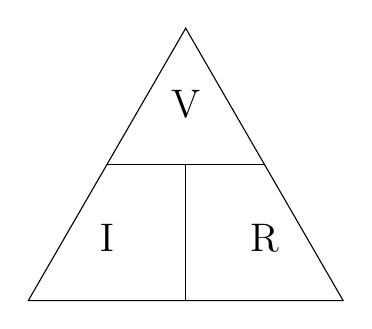
\begin{tikzpicture}
    \draw (0,0) -- (4,0) -- (2,3.46) -- cycle;
    \draw (1,1.73) -- (3,1.73);
    \draw (2,1.73) -- (2,0);
    \node at (2,2.5) {\Large V};
    \node at (1,0.8) {\Large I};
    \node at (3,0.8) {\Large R};
\end{tikzpicture}
\end{answerdiagram}
\end{solutionbox}

\begin{mnemonicbox}
\mnemonic{Volts Invite current, Resistance Restricts}
\end{mnemonicbox}

\questionmarks{2(c) OR}{7}{Show that the current in a purely capacitive circuit leads the applied voltage by 90$^{\circ}$ and the current in a purely inductive circuit lags the applied voltage by 90$^{\circ}$.}

\begin{solutionbox}
\textbf{Answer}:

\textbf{For Capacitive Circuit:}
\begin{itemize}
    \item Voltage equation: $v = V_m \sin(\omega t)$
    \item Current: $i = C \frac{dv}{dt} = \omega C V_m \cos(\omega t) = I_m \sin(\omega t + 90^\circ)$
    \item \textbf{Result:} Current leads voltage by 90$^\circ$
\end{itemize}

\textbf{For Inductive Circuit:}
\begin{itemize}
    \item Voltage equation: $v = L \frac{di}{dt}$
    \item Integrating voltage gives current: $i = -\frac{V_m}{\omega L} \cos(\omega t) = I_m \sin(\omega t - 90^\circ)$
    \item \textbf{Result:} Current lags voltage by 90$^\circ$
\end{itemize}

\begin{answerdiagram}{Phase Relationships}
\begin{tikzpicture}[scale=0.8]
    % Capacitor
    \begin{scope}[xshift=0cm]
        \draw[->] (0,0) -- (2,0) node[right] {$V$};
        \draw[->] (0,0) -- (0,2) node[above] {$I$};
        \node at (1,-1) {Capacitor (Lead)};
    \end{scope}

    % Inductor
    \begin{scope}[xshift=4cm]
        \draw[->] (0,0) -- (2,0) node[right] {$V$};
        \draw[->] (0,0) -- (0,-2) node[below] {$I$};
        \node at (1,-1) {Inductor (Lag)};
    \end{scope}
\end{tikzpicture}
\end{answerdiagram}
\end{solutionbox}

\begin{mnemonicbox}
\mnemonic{ELI the ICE man - In EL (inductor), I lags E; in ICE (capacitor), I leads E}
\end{mnemonicbox}

% Question 3
\questionmarks{3(a)}{3}{Define cycle, form factor and amplitude.}

\begin{solutionbox}
\textbf{Answer}:

\begin{itemize}
    \item \keyword{Cycle}: One complete repetition of a waveform.
    \item \keyword{Form Factor}: Ratio of RMS value to average value. For sine wave = 1.11.
    \item \keyword{Amplitude}: Maximum displacement of a waveform from its mean position.
\end{itemize}

\begin{answerdiagram}{Waveform Definitions}
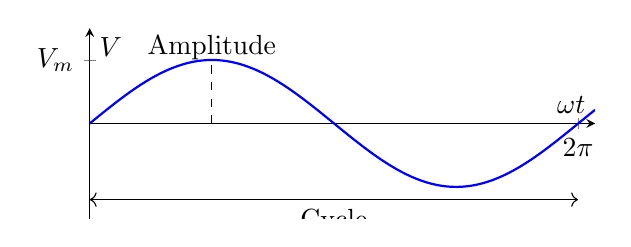
\begin{tikzpicture}
    \begin{axis}[
        width=8cm, height=4cm,
        axis lines=middle,
        xtick={0, 6.28},
        xticklabels={0, $2\pi$},
        ytick={1},
        yticklabels={$V_m$},
        xlabel=$\omega t$,
        ylabel=$V$,
        ymin=-1.5, ymax=1.5
    ]
    \addplot[blue, thick, domain=0:6.5, samples=100] {sin(deg(x))};
    \draw[<->] (axis cs:0,-1.2) -- (axis cs:6.28,-1.2) node[midway, below] {Cycle};
    \draw[dashed] (axis cs:1.57,0) -- (axis cs:1.57,1);
    \node at (axis cs:1.57,1.2) {Amplitude};
    \end{axis}
\end{tikzpicture}
\end{answerdiagram}
\end{solutionbox}

\begin{mnemonicbox}
\mnemonic{Cycles Complete, Form Factors Find ratio, Amplitude Achieves maximum}
\end{mnemonicbox}

\questionmarks{3(b)}{4}{Define RMS and Average value. Write expression of RMS and average value of sinusoidal waveform.}

\begin{solutionbox}
\textbf{Answer}:

\begin{center}
\captionof{table}{RMS vs Average Value}
\begin{tabulary}{\linewidth}{|L|L|L|}
\hline
\textbf{Parameter} & \textbf{Definition} & \textbf{Formula for Sine Wave} \\ \hline
\textbf{RMS Value} & Square root of mean of squared values & $V_{rms} = V_m/\sqrt{2} = 0.707 V_m$ \\ \hline
\textbf{Average Value} & Mean of all instantaneous values over half cycle & $V_{avg} = 2V_m/\pi = 0.637 V_m$ \\ \hline
\end{tabulary}
\end{center}

\begin{itemize}
    \item \keyword{RMS (Root Mean Square)}: Equivalent DC value that produces same heating effect.
    \item \keyword{Average Value}: Mean of all instantaneous values over a half cycle.
\end{itemize}
\end{solutionbox}

\begin{mnemonicbox}
\mnemonic{RMS Relates to heating, Average Adds and divides}
\end{mnemonicbox}

\questionmarks{3(c)}{7}{Explain the terms Apparent power, True Power and Reactive power. State their unit of measurement.}

\begin{solutionbox}
\textbf{Answer}:

\begin{center}
\captionof{table}{Types of Power}
\begin{tabulary}{\linewidth}{|L|L|L|L|}
\hline
\textbf{Power Type} & \textbf{Definition} & \textbf{Formula} & \textbf{Unit} \\ \hline
\textbf{Apparent Power (S)} & Total power supplied & $S = VI$ & VA (Volt-Ampere) \\ \hline
\textbf{True Power (P)} & Actual power consumed & $P = VI \cos \phi$ & W (Watt) \\ \hline
\textbf{Reactive Power (Q)} & Power oscillating between source and load & $Q = VI \sin \phi$ & VAR (Volt-Ampere Reactive) \\ \hline
\end{tabulary}
\end{center}

\keyword{Power Triangle:} $S^2 = P^2 + Q^2$

\begin{answerdiagram}{Power Triangle}
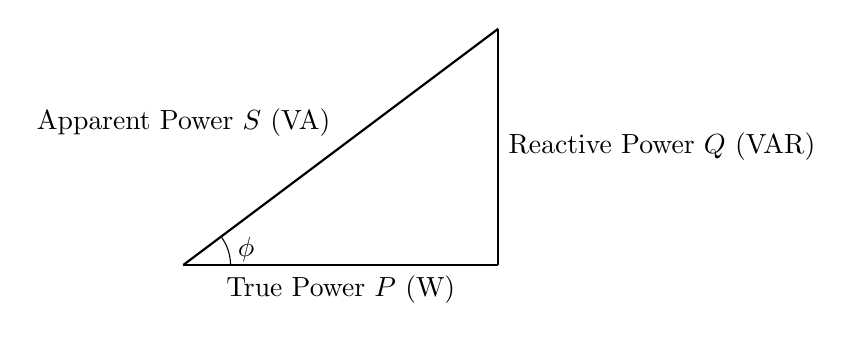
\begin{tikzpicture}
    \draw[thick] (0,0) -- (4,0) node[midway, below] {True Power $P$ (W)};
    \draw[thick] (4,0) -- (4,3) node[midway, right] {Reactive Power $Q$ (VAR)};
    \draw[thick] (0,0) -- (4,3) node[midway, above left] {Apparent Power $S$ (VA)};
    \draw (0.6,0) arc (0:36.87:0.6) node[midway, right] {$\phi$};
\end{tikzpicture}
\end{answerdiagram}
\end{solutionbox}

\begin{mnemonicbox}
\mnemonic{Active Performs work, Reactive Returns energy, Apparent Adds vectors}
\end{mnemonicbox}

% Question 3 OR
\questionmarks{3(a) OR}{3}{Write mathematical expressions of 3-phase voltages.}

\begin{solutionbox}
\textbf{Answer}:

\textbf{Three-phase voltage expressions:}

\begin{center}
\captionof{table}{3-Phase Voltages}
\begin{tabulary}{\linewidth}{|L|L|}
\hline
\textbf{Phase} & \textbf{Expression} \\ \hline
\textbf{R-phase} & $V_R = V_m \sin(\omega t)$ \\ \hline
\textbf{Y-phase} & $V_Y = V_m \sin(\omega t - 120^\circ)$ \\ \hline
\textbf{B-phase} & $V_B = V_m \sin(\omega t - 240^\circ)$ \\ \hline
\end{tabulary}
\end{center}

Where $V_m$ is the maximum voltage and $\omega$ is the angular frequency.
\end{solutionbox}

\begin{mnemonicbox}
\mnemonic{Red phase Reference, Yellow lags 120, Blue brings up 240}
\end{mnemonicbox}

\questionmarks{3(b) OR}{4}{Define crest factor and state value of crest factor for sine wave.}

\begin{solutionbox}
\textbf{Answer}:

\begin{itemize}
    \item \keyword{Crest Factor}: Ratio of peak value to RMS value of a waveform.
    \item \keyword{Formula}: $\text{Crest Factor} = \frac{\text{Peak Value}}{\text{RMS Value}}$
    \item \keyword{For sine wave}: $\text{Crest Factor} = \frac{1}{0.707} = 1.414$
\end{itemize}

\begin{answerdiagram}{Crest Factor Concept}
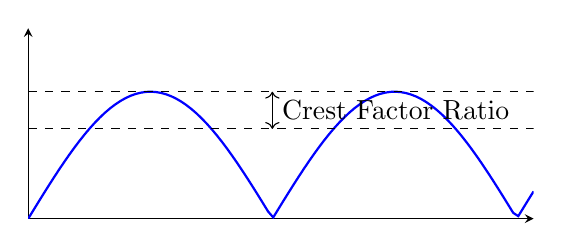
\begin{tikzpicture}
    \begin{axis}[
        width=8cm, height=4cm,
        axis lines=middle,
        xtick=\empty, ytick=\empty,
        ymin=0, ymax=1.5,
        xmin=0, xmax=6.5
    ]
    \addplot[blue, thick, domain=0:6.5, samples=100] {abs(sin(deg(x)))};
    \draw[dashed] (axis cs:0,1) -- (axis cs:6.5,1) node[right] {Peak};
    \draw[dashed] (axis cs:0,0.707) -- (axis cs:6.5,0.707) node[right] {RMS};
    \draw[<->] (axis cs:3.14, 0.707) -- (axis cs:3.14, 1) node[midway, right] {Crest Factor Ratio};
    \end{axis}
\end{tikzpicture}
\end{answerdiagram}
\end{solutionbox}

\begin{mnemonicbox}
\mnemonic{Crest Compares peak to RMS}
\end{mnemonicbox}

\questionmarks{3(c) OR}{7}{Describe different three phase electrical connections.}

\begin{solutionbox}
\textbf{Answer}:

\begin{center}
\captionof{table}{Star vs Delta Connection}
\begin{tabulary}{\linewidth}{|L|L|L|}
\hline
\textbf{Parameter} & \textbf{Star (Y) Connection} & \textbf{Delta ($\Delta$) Connection} \\ \hline
\textbf{Line Voltage ($V_L$)} & $\sqrt{3} \times \text{Phase Voltage}$ & Same as Phase Voltage \\ \hline
\textbf{Line Current ($I_L$)} & Same as Phase Current & $\sqrt{3} \times \text{Phase Current}$ \\ \hline
\textbf{Neutral Wire} & Present & Absent \\ \hline
\textbf{Application} & Unbalanced loads, Residential & Balanced loads, Industrial \\ \hline
\end{tabulary}
\end{center}

\begin{answerdiagram}{Star and Delta Connections}
\begin{circuitikz}[scale=0.7, transform shape]
    % Star
    \draw (0,0) node[anchor=north]{N} to[R, l=R] (0,2) node[anchor=south]{R};
    \draw (0,0) to[R, l=Y] (-1.73,-1) node[anchor=north]{Y};
    \draw (0,0) to[R, l=B] (1.73,-1) node[anchor=north]{B};
    \node at (0,-2.5) {Star Connection};

    % Delta
    \begin{scope}[xshift=5cm, yshift=-1cm]
    \draw (0,0) to[R, l=B] (4,0);
    \draw (0,0) to[R, l=R] (2,3.46);
    \draw (2,3.46) to[R, l=Y] (4,0);
    \node at (2,-1.5) {Delta Connection};
    \end{scope}
\end{circuitikz}
\end{answerdiagram}
\end{solutionbox}

\begin{mnemonicbox}
\mnemonic{Star Shows neutral, Delta Delivers higher current}
\end{mnemonicbox}

% Question 4
\questionmarks{4(a)}{3}{Calculate the peak to peak value of a sinusoidal voltage if RMS value is 230V.}

\begin{solutionbox}
\textbf{Answer}:

\begin{center}
\captionof{table}{Calculation Steps}
\begin{tabulary}{\linewidth}{|L|L|L|}
\hline
\textbf{Parameter} & \textbf{Formula} & \textbf{Calculation} \\ \hline
\textbf{RMS Value} & Given & 230V \\ \hline
\textbf{Peak Value} & $V_m = \sqrt{2} \times V_{rms}$ & $V_m = \sqrt{2} \times 230 = 325.27\text{V}$ \\ \hline
\textbf{Peak-to-Peak} & $V_{p-p} = 2 \times V_m$ & $V_{p-p} = 2 \times 325.27 = 650.54\text{V}$ \\ \hline
\end{tabulary}
\end{center}

\textbf{Therefore, peak-to-peak value = 650.54V}
\end{solutionbox}

\begin{mnemonicbox}
\mnemonic{RMS to Peak - multiply by root2, Peak to Peak - double it}
\end{mnemonicbox}

\questionmarks{4(b)}{4}{An alternating current is given by i=142.14sin628t find frequency and time period.}

\begin{solutionbox}
\textbf{Answer}:

\textbf{Given equation:} $i = 142.14 \sin(628t)$ implies $\omega = 628$ rad/s.

\begin{center}
\captionof{table}{Calculation Steps}
\begin{tabulary}{\linewidth}{|L|L|L|}
\hline
\textbf{Parameter} & \textbf{Formula} & \textbf{Calculation} \\ \hline
\textbf{Frequency} & $f = \omega/(2\pi)$ & $f = 628/(2\pi) = 100 \text{ Hz}$ \\ \hline
\textbf{Time Period} & $T = 1/f$ & $T = 1/100 = 0.01 \text{ s} = 10 \text{ ms}$ \\ \hline
\end{tabulary}
\end{center}

\textbf{Therefore, frequency = 100 Hz and time period = 0.01 s}
\end{solutionbox}

\begin{mnemonicbox}
\mnemonic{Frequency From omega divide 2pi, Time takes inverse}
\end{mnemonicbox}

\questionmarks{4(c)}{7}{State and explain Fleming's left hand rule and right hand rule.}

\begin{solutionbox}
\textbf{Answer}:

\begin{itemize}
    \item \keyword{Fleming's Left Hand Rule (Motor):}
    \begin{itemize}
        \item Used to determine direction of \textbf{force} on a current-carrying conductor in a magnetic field.
        \item Thumb: Motion (Force)
        \item Forefinger: Magnetic field
        \item Middle finger: Current
    \end{itemize}

    \item \keyword{Fleming's Right Hand Rule (Generator):}
    \begin{itemize}
        \item Used to determine direction of \textbf{induced current} when a conductor moves in a magnetic field.
        \item Thumb: Motion of conductor
        \item Forefinger: Magnetic field
        \item Middle finger: Induced current
    \end{itemize}
\end{itemize}

\begin{answerdiagram}{Fleming's Rules Hand Positions}
\begin{tikzpicture}
    % Left Hand
    \begin{scope}[xshift=0cm]
        \draw[->, Ultra Thick, blue] (0,0) -- (0,2) node[above] {Motion};
        \draw[->, Ultra Thick, red] (0,0) -- (2,0) node[right] {Field};
        \draw[->, Ultra Thick, green!60!black] (0,0) -- (0,0,-2) node[left] {Current};
        \node at (0,-1) {Left Hand (Motor)};
    \end{scope}
    
    % Right Hand
    \begin{scope}[xshift=5cm]
        \draw[->, Ultra Thick, blue] (0,0) -- (0,2) node[above] {Motion};
        \draw[->, Ultra Thick, red] (0,0) -- (2,0) node[right] {Field};
        \draw[->, Ultra Thick, purple] (0,0) -- (0,0,-2) node[left] {Induced Current};
        \node at (0,-1) {Right Hand (Generator)};
    \end{scope}
\end{tikzpicture}
\end{answerdiagram}
\end{solutionbox}

\begin{mnemonicbox}
\mnemonic{Left Lifts motors, Right Raises generators}
\end{mnemonicbox}

% Question 4 OR
\questionmarks{4(a) OR}{3}{A conductor of length 1 metre moves with speed of 30m/s in magnetic field of 0.6 Tesla making angle of 30$^{\circ}$ with the field. Calculate dynamically EMF induced in it. (use sin 30$^{\circ}$=0.5)}

\begin{solutionbox}
\textbf{Answer}:

\begin{center}
\captionof{table}{Given Parameters}
\begin{tabulary}{\linewidth}{|L|L|}
\hline
\textbf{Parameter} & \textbf{Value} \\ \hline
\textbf{Length (l)} & 1 meter \\ \hline
\textbf{Speed (v)} & 30 m/s \\ \hline
\textbf{Magnetic Field (B)} & 0.6 Tesla \\ \hline
\textbf{Angle ($\theta$)} & $30^\circ$ \\ \hline
\end{tabulary}
\end{center}

\keyword{Formula:} $E = Blv \sin \theta$

\textbf{Calculation:}
\[ E = 0.6 \times 1 \times 30 \times 0.5 = 9 \text{ volts} \]

\textbf{Therefore, induced EMF = 9 volts}
\end{solutionbox}

\begin{mnemonicbox}
\mnemonic{EMF Emerges from Field, velocity and Length with angle}
\end{mnemonicbox}

\questionmarks{4(b) OR}{4}{State \& explain Lenz's law.}

\begin{solutionbox}
\textbf{Answer}:

\keyword{Lenz's Law:} The direction of induced EMF or current is always such that it opposes the cause that produces it.

\keyword{Application:} When a magnet approaches a coil, induced current creates a magnetic field that repels the approaching magnet.

\begin{answerdiagram}{Lenz's Law}
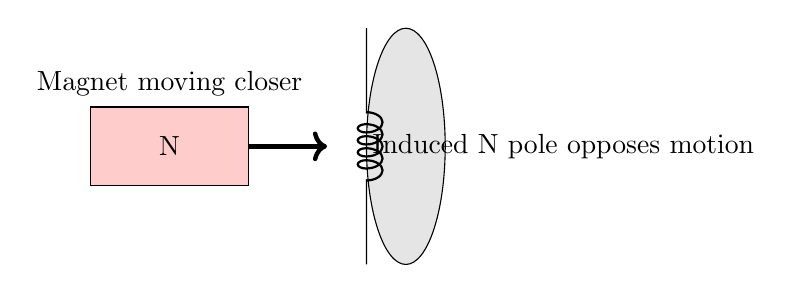
\begin{tikzpicture}
    \draw[fill=gray!20] (0,0) circle (0.5 and 1.5);
    \draw (-0.5,1.5) to[L] (-0.5, -1.5); % Coil representation
    \draw[->, ultra thick] (-2,0) -- (-1,0); 
    \draw[fill=red!20] (-4,-0.5) rectangle (-2,0.5) node[midway] {N};
    \node at (-3, 0.8) {Magnet moving closer};
    \node at (2,0) {Induced N pole opposes motion};
\end{tikzpicture}
\end{answerdiagram}
\end{solutionbox}

\begin{mnemonicbox}
\mnemonic{Lenz Likes to Oppose}
\end{mnemonicbox}

\questionmarks{4(c) OR}{7}{Explain Statically and dynamically induced EMF.}

\begin{solutionbox}
\textbf{Answer}:

\begin{center}
\captionof{table}{Statically vs Dynamically Induced EMF}
\begin{tabulary}{\linewidth}{|L|L|L|}
\hline
\textbf{Parameter} & \textbf{Statically Induced EMF} & \textbf{Dynamically Induced EMF} \\ \hline
\textbf{Definition} & EMF induced due to change in current/flux & EMF induced due to movement of conductor in magnetic field \\ \hline
\textbf{Physical Action} & Fixed conductor, changing field & Moving conductor in fixed field \\ \hline
\textbf{Example} & Transformer & Generator \\ \hline
\textbf{Formula} & $e = -N \frac{d\Phi}{dt}$ & $e = Blv \sin \theta$ \\ \hline
\end{tabulary}
\end{center}
\end{solutionbox}

\begin{mnemonicbox}
\mnemonic{Static Stays but flux Changes, Dynamic Drives through field}
\end{mnemonicbox}

% Question 5
\questionmarks{5(a)}{3}{Explain PV Cell.}

\begin{solutionbox}
\textbf{Answer}:

\begin{itemize}
    \item \keyword{PV Cell}: Device that converts sunlight directly into electricity using photovoltaic effect.
    \item \keyword{Working}: Sunlight excites electrons in semiconductor material, creating voltage difference.
    \item \keyword{Material}: Typically made from silicon with P-N junction.
\end{itemize}

\begin{answerdiagram}{PV Cell Structure}
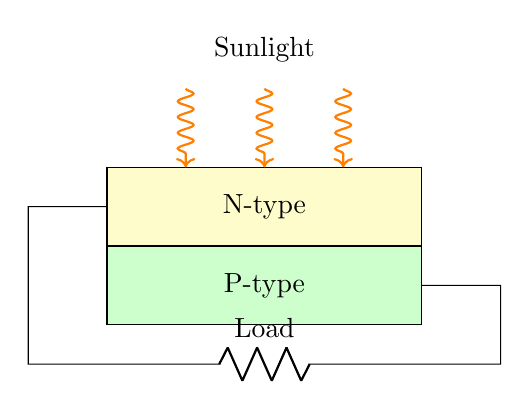
\begin{tikzpicture}
    \draw[fill=yellow!20] (0,1) rectangle (4,2) node[midway] {N-type};
    \draw[fill=green!20] (0,0) rectangle (4,1) node[midway] {P-type};
    \foreach \x in {1,2,3} \draw[->, decorate, decoration={snake, amplitude=1mm, segment length=2mm, post length=1mm}, thick, orange] (\x,3) -- (\x,2);
    \node at (2,3.5) {Sunlight};
    \draw (0,1.5) -- (-1,1.5) -- (-1,-0.5) to[R, l=Load] (5,-0.5) -- (5,0.5) -- (4,0.5);
\end{tikzpicture}
\end{answerdiagram}
\end{solutionbox}

\begin{mnemonicbox}
\mnemonic{Photons Visit, Current Created}
\end{mnemonicbox}

\questionmarks{5(b)}{4}{Explain the solar PV panel and arrays.}

\begin{solutionbox}
\textbf{Answer}:

\begin{center}
\captionof{table}{Solar System Hierarchy}
\begin{tabulary}{\linewidth}{|L|L|}
\hline
\textbf{Component} & \textbf{Description} \\ \hline
\textbf{PV Cell} & Basic unit that converts sunlight to electricity (0.5V - 0.6V) \\ \hline
\textbf{PV Panel} & Multiple cells connected in series/parallel (typically 12V, 24V) \\ \hline
\textbf{PV Array} & Multiple panels connected to achieve required voltage/current \\ \hline
\end{tabulary}
\end{center}

\begin{answerdiagram}{Cell to Array Hierarchy}
\begin{tikzpicture}[node distance=1.5cm, auto]
    \node [gtu block] (Cell) {Solar Cell};
    \node [gtu block, right=of Cell] (Panel) {Solar Panel};
    \node [gtu block, right=of Panel] (Array) {Solar Array};
    \draw [gtu arrow] (Cell) -- node{Series Connection} (Panel);
    \draw [gtu arrow] (Panel) -- node{Matrix Connection} (Array);
\end{tikzpicture}
\end{answerdiagram}
\end{solutionbox}

\begin{mnemonicbox}
\mnemonic{Cells Combine into Panels, Panels Produce Arrays}
\end{mnemonicbox}

\questionmarks{5(c)}{7}{Draw and explain block diagram of wind power system.}

\begin{solutionbox}
\textbf{Answer}:

\textbf{Components of Wind Power System:}
\begin{enumerate}
    \item \keyword{Wind Turbine}: Converts wind energy to mechanical energy
    \item \keyword{Gearbox}: Increases rotational speed for generator
    \item \keyword{Generator}: Converts mechanical energy to electrical energy
    \item \keyword{Power Electronics}: Controls and regulates electrical output
    \item \keyword{Transformer}: Steps up/down voltage for transmission/distribution
    \item \keyword{Control System}: Monitors and optimizes overall operation
\end{enumerate}

\begin{answerdiagram}{Wind Power System Block Diagram}
\begin{tikzpicture}[node distance=1.2cm, auto]
    \node [gtu block] (W) {Wind};
    \node [gtu block, right=0.5cm of W] (T) {Turbine};
    \node [gtu block, right=0.5cm of T] (G) {Gearbox};
    \node [gtu block, right=0.5cm of G] (Gen) {Generator};
    \node [gtu block, right=0.5cm of Gen] (PE) {Power\\Electronics};
    \node [gtu block, below=0.8cm of PE] (Tr) {Transformer};
    \node [gtu block, left=0.5cm of Tr] (Grid) {Grid};
    
    \path [gtu arrow] (W) -- (T);
    \path [gtu arrow] (T) -- (G);
    \path [gtu arrow] (G) -- (Gen);
    \path [gtu arrow] (Gen) -- (PE);
    \path [gtu arrow] (PE) -- (Tr);
    \path [gtu arrow] (Tr) -- (Grid);
\end{tikzpicture}
\end{answerdiagram}
\end{solutionbox}

\begin{mnemonicbox}
\mnemonic{Wind Turns Gears, Generating Electrical Returns}
\end{mnemonicbox}

% Question 5 OR
\questionmarks{5(a) OR}{3}{State the benefits of green energy.}

\begin{solutionbox}
\textbf{Answer}:

\begin{center}
\captionof{table}{Benefits of Green Energy}
\begin{tabulary}{\linewidth}{|L|L|}
\hline
\textbf{Benefit Category} & \textbf{Examples} \\ \hline
\textbf{Environmental} & Reduces pollution, Minimizes carbon footprint \\ \hline
\textbf{Economic} & Creates jobs, Reduces energy dependency \\ \hline
\textbf{Health} & Improves air quality, Reduces health issues \\ \hline
\textbf{Sustainability} & Renewable, Inexhaustible sources \\ \hline
\end{tabulary}
\end{center}
\end{solutionbox}

\begin{mnemonicbox}
\mnemonic{Clean Energy Creates Economic Salvation}
\end{mnemonicbox}

\questionmarks{5(b) OR}{4}{Explain Solar PV applications in brief.}

\begin{solutionbox}
\textbf{Answer}:

\textbf{Solar PV Applications:}
\begin{enumerate}
    \item \keyword{Residential}: Rooftop systems, Solar water heaters
    \item \keyword{Commercial}: Building integrated PV, Solar parking
    \item \keyword{Industrial}: Process heating, Power generation
    \item \keyword{Utility Scale}: Solar farms, Grid support
    \item \keyword{Off-grid}: Rural electrification, Remote applications
\end{enumerate}

\begin{answerdiagram}{Solar PV Applications}
\begin{tikzpicture}[
  level 1/.style={sibling distance=2.5cm},
  level 2/.style={sibling distance=1.5cm}
]
\node [gtu root] {Solar PV}
    child { node [gtu child] {Residential} }
    child { node [gtu child] {Commercial} }
    child { node [gtu child] {Industrial} }
    child { node [gtu child] {Utility} }
    child { node [gtu child] {Off-grid} };
\end{tikzpicture}
\end{answerdiagram}
\end{solutionbox}

\begin{mnemonicbox}
\mnemonic{Residences, Commerce, Industry Utilize Solar}
\end{mnemonicbox}

\questionmarks{5(c) OR}{7}{Explain different types of Green energy.}

\begin{solutionbox}
\textbf{Answer}:

\begin{center}
\captionof{table}{Types of Green Energy}
\begin{tabulary}{\linewidth}{|L|L|L|}
\hline
\textbf{Type} & \textbf{Source} & \textbf{Applications} \\ \hline
\textbf{Solar} & Sun & PV systems, Thermal plants \\ \hline
\textbf{Wind} & Moving air & Wind turbines, Windmills \\ \hline
\textbf{Hydro} & Flowing water & Dams, Run-of-river systems \\ \hline
\textbf{Biomass} & Organic matter & Combustion, Biogas production \\ \hline
\textbf{Geothermal} & Earth's heat & Direct heating, Power plants \\ \hline
\textbf{Tidal} & Ocean tides & Barrage systems, Tidal turbines \\ \hline
\end{tabulary}
\end{center}

\begin{answerdiagram}{Green Energy Sources Distribution}
\begin{tikzpicture}
    \pie[radius=2, text=pin, color={yellow!40, blue!20, cyan!30, green!30, orange!30, purple!30}]{
        30/Solar,
        25/Wind,
        20/Hydro,
        15/Biomass,
        7/Geothermal,
        3/Tidal
    }
\end{tikzpicture}
\end{answerdiagram}
\end{solutionbox}

\begin{mnemonicbox}
\mnemonic{Sun, Wind, Hydro, Biomass, Geothermal, Tidal}
\end{mnemonicbox}

\end{document}


